\documentclass[10pt,a4paper]{article}
\usepackage[a4paper, top=1.5cm, bottom=1.5cm, left=1.5cm, right=1.5cm]{geometry}
\usepackage{amsmath, amssymb}
\usepackage[version=4]{mhchem}
\usepackage{multicol}
\usepackage{enumitem}
\usepackage{array}
\usepackage{booktabs}
\usepackage{tabularx}
\usepackage{xcolor}
\usepackage{mdframed}
\usepackage{titlesec}
\usepackage{fancyhdr}
\usepackage{parskip}
\usepackage{fontenc}
\usepackage{inputenc}
\usepackage{tikz}
\usepackage{graphicx}

% Colors
\definecolor{darkblue}{RGB}{0,0,128}
\definecolor{sectionbg}{RGB}{30,30,80}
\definecolor{ncertbg}{RGB}{220,220,220}

% Page style
\pagestyle{fancy}
\fancyhf{}
\fancyhead[L]{\textbf{Chemistry}}
\fancyhead[R]{\textbf{Redox Reactions}}
\fancyfoot[C]{\thepage}
\renewcommand{\headrulewidth}{0.4pt}

% Section formatting
\titleformat{\section}[block]{\color{white}\bfseries\large\centering}{}{0em}{}
\titlespacing{\section}{0pt}{6pt}{4pt}

% Custom environments
\newenvironment{sectionbox}[1]{%
  \begin{mdframed}[backgroundcolor=sectionbg, linewidth=0pt, innerleftmargin=6pt, innerrightmargin=6pt, innertopmargin=4pt, innerbottommargin=4pt]
  \color{white}\bfseries\centering #1
  \end{mdframed}
}{}

\newenvironment{ncertbox}{%
  \begin{mdframed}[backgroundcolor=ncertbg, linewidth=0.5pt, innerleftmargin=6pt, innerrightmargin=6pt, innertopmargin=3pt, innerbottommargin=3pt]
  \textbf{NCERT Based}
  \end{mdframed}
}{}

% Question list style
\newlist{questions}{enumerate}{1}
\setlist[questions]{label=\textbf{\arabic*.}, leftmargin=*, itemsep=2pt, parsep=0pt, topsep=4pt}

\newlist{options}{enumerate}{1}
\setlist[options]{label=(\arabic*), leftmargin=2em, itemsep=0pt, parsep=0pt, topsep=2pt}

\newlist{optionsA}{enumerate}{1}
\setlist[optionsA]{label=(\arabic*), leftmargin=2em, itemsep=0pt, parsep=0pt, topsep=2pt}

% For inline options in 2-column
\newcommand{\opt}[4]{%
\begin{multicols}{2}
\begin{options}
  \item #1
  \item #2
  \item #3
  \item #4
\end{options}
\end{multicols}
}

\setlength{\columnseprule}{0.3pt}
\setlength{\columnsep}{12pt}

\begin{document}

\begin{center}
  {\Large\textbf{TOPICWISE QUESTIONS}}\\[4pt]
  {\small NCERT Based}
\end{center}

% ============================================================
\begin{mdframed}[backgroundcolor=sectionbg, linewidth=0pt, innerleftmargin=6pt, innerrightmargin=6pt, innertopmargin=4pt, innerbottommargin=4pt]
\color{white}\bfseries\small REDOX REACTIONS: CLASSICAL IDEA, IN TERMS OF ELECTRON TRANSFER, TYPES OF REDOX REACTIONS
\end{mdframed}

\begin{multicols}{2}
\begin{questions}

\item In which of the following reactions, hydrogen is acting as an oxidising agent?
\begin{options}
  \item With Li to form \ce{LiH}
  \item With \ce{I2} to give \ce{HI}
  \item With S to give \ce{H2S}
  \item None of the above
\end{options}

\item Which of the following acts as an oxidising as well as reducing agent?
\begin{options}
  \item \ce{Na2O}
  \item \ce{Na2O2}
  \item \ce{NaNO3}
  \item \ce{NaNO2}
\end{options}

\item Which quantities are conserved in all oxidation-reduction reactions?
\begin{options}
  \item Charge only
  \item Mass only
  \item Both charge and mass
  \item Neither charge nor mass
\end{options}

\item In the reaction, \ce{SO2 + 2H2S -> 3S + 2H2O}, the substance oxidised is
\begin{options}
  \item \ce{H2S}
  \item \ce{SO2}
  \item S
  \item \ce{H2O}
\end{options}

\item In which of the following reactions, chlorine acts as an oxidising agent?
\begin{options}[topsep=2pt]
  \item[] (i) \ce{CH3CH2OH + Cl2 -> CH3CHO + HCl}
  \item[] (ii) \ce{CH3CHO + Cl2 -> CCl3CHO + HCl}
  \item[] (iii) \ce{CH4 + Cl2 -> CH3Cl + HCl}
\end{options}
The correct answer is
\begin{options}
  \item (i) only
  \item (ii) only
  \item (i) and (iii)
  \item (i), (ii) and (iii)
\end{options}

\item Which of the following is not a redox reaction?
\begin{options}
  \item \ce{2Na + Cl2 -> 2NaCl}
  \item \ce{C + O2 -> CO2}
  \item \ce{AgNO3 + NaCl -> NaNO3 + AgCl}
  \item \ce{Zn + H2SO4 -> ZnSO4 + H2}
\end{options}

\item In the reaction, \ce{H2O2 + Na2CO3 -> Na2O2 + CO2 + H2O} the substance undergoing oxidation is
\begin{options}
  \item \ce{H2O2}
  \item \ce{Na2CO3}
  \item \ce{Na2O2}
  \item None of these
\end{options}

\item In the following reaction, \ce{4P + 3KOH + 3H2O -> 3KH2PO2 + PH3}
\begin{options}
  \item P is only oxidized
  \item P is only reduced
  \item P is both oxidized as well as reduced
  \item P is neither oxidized nor reduced
\end{options}

\item In which reaction, the underlined substance has been reduced?
\begin{options}
  \item \underline{Carbon monoxide} + copper oxide $\to$ carbon dioxide + copper
  \item \underline{Copper oxide} + hydrochloric acid $\to$ water + copper chloride
  \item \underline{Steam} + iron $\to$ hydrogen + iron oxide
  \item \underline{Hydrogen} + iron oxide $\to$ water + iron
\end{options}

\item Bleaching action of \ce{SO2} is due to:
\begin{options}
  \item Reduction
  \item Oxidation
  \item Hydrolysis
  \item Acidic nature
\end{options}

\item In the preparation of chlorine from \ce{HCl}, \ce{MnO2} acts as:
\begin{options}
  \item Reducing agent
  \item Oxidising agent
  \item Catalytic agent
  \item Dehydrating agent
\end{options}

\item Sulphurous acid can be used as:
\begin{options}
  \item Oxidising agent
  \item Reducing agent
  \item Bleaching agent
  \item All of these
\end{options}

\item Stannous chloride gives a white precipitate with a solution of mercuric chloride. In this process, mercuric chloride is:
\begin{options}
  \item Oxidized
  \item Reduced
  \item Converted into a complex compound containing Sn and Hg
  \item Converted into a chloro complex of Hg
\end{options}

\item Oxidants are substances which:
\begin{options}
  \item Show a decrease in their oxidation number during a change
  \item Gain electrons during a change
  \item Oxidise others and reduce themselves
  \item All of the above
\end{options}

\item In which \ce{SO2} acts as oxidant, while reacting with:
\begin{options}
  \item Acidified \ce{KMnO4}
  \item Acidified \ce{K2Cr2O7}
  \item \ce{H2S}
  \item Acidified \ce{C2H5OH}
\end{options}

\item Which is not an oxidising agent?
\begin{options}
  \item \ce{KClO3}
  \item \ce{O2}
  \item \ce{C6H12O6}
  \item \ce{K2Cr2O7}
\end{options}

\item Respiration is an example of
\begin{options}
  \item Oxidation
  \item Reduction
  \item Both (1) and (2)
  \item Combination
\end{options}

\item Magnesium reacts with acids producing hydrogen and corresponding magnesium salts. In such reactions, magnesium undergoes:
\begin{options}
  \item Oxidation
  \item Reduction
  \item Neither oxidation nor reduction
  \item Simple dissolution
\end{options}

\item \ce{LiAlH4} is used as:
\begin{options}
  \item Oxidising agent
  \item Reducing agent
  \item A mordant
  \item Water softener
\end{options}

\item A sulphur containing species that cannot be an oxidising agent is:
\begin{options}
  \item \ce{H2SO4}
  \item \ce{H2S}
  \item \ce{SO2}
  \item \ce{H2SO3}
\end{options}

\item Which statement is incorrect?
\begin{options}
  \item Oxidation of a substance is followed by reduction of another.
  \item Reduction of a substance is followed by oxidation of another.
  \item Oxidation and reduction are complementary reactions.
  \item It is not necessary that both oxidation and reduction should take place in the same reaction.
\end{options}

\item In \ce{C + H2O -> CO + H2}; \ce{H2O} acts as:
\begin{options}
  \item Oxidant
  \item Reductant
  \item Both (1) and (2)
  \item Catalyst
\end{options}

\item In \ce{N2 + 2H2O -> NH4+ + NO2-}; N is:
\begin{options}
  \item Oxidised
  \item Reduced
  \item Both (1) and (2)
  \item Neither (1) nor (2)
\end{options}

\item Fluorine is a strong oxidising agent because:
\begin{options}
  \item It has several isotopes
  \item It is very small and has 7 electrons in valence shell
  \item Its valency is one
  \item It is the first member of the halogen series
\end{options}

\item Reductants are substances which:
\begin{options}
  \item Show an increase in their oxidation number during a change
  \item Lose electrons during a change
  \item Reduce others and oxidise themselves
  \item All of the above
\end{options}

\item Stronger is oxidising agent, more is;
\begin{options}
  \item Standard reduction potential of that species
  \item The tendency to get itself oxidised
  \item The tendency to lose electrons by that species
  \item Standard oxidation potential of that species
\end{options}

\item Corrosion of iron is:
\begin{options}
  \item Oxidation process
  \item Neutralization process
  \item Precipitation process
  \item Combination process
\end{options}

\item Which conversion is an oxidation reaction?
\begin{options}
  \item \ce{SO4^{2-} -> SO3^{2-}}
  \item \ce{Cu^{2+} -> Cu}
  \item \ce{H+ -> H}
  \item \ce{H- -> H}
\end{options}

\item Which of the following reaction involves oxidation and reduction?
\begin{options}
  \item \ce{NaBr + HCl -> NaCl + HBr}
  \item \ce{HBr + AgNO3 -> AgBr + HNO3}
  \item \ce{H2 + Br2 -> 2HBr}
  \item \ce{Na2O + H2SO4 -> Na2SO4 + H2O}
\end{options}

\item How many electrons are involved in reduction of \ce{KMnO4} in basic medium?
\begin{options}
  \item 1
  \item 2
  \item 5
  \item 3
\end{options}

\item The number of electrons lost or gained during the change \ce{Fe + H2O -> Fe3O4 + H2} is
\begin{options}
  \item 2
  \item 4
  \item 6
  \item 8
\end{options}

\item Which change occur when lead monoxide is converted into lead nitrate?
\begin{options}
  \item Oxidation
  \item Reduction
  \item Neither oxidation nor reduction
  \item Both oxidation and reduction
\end{options}

\item In the reaction, \ce{C + 4HNO3 -> CO2 + 2H2O + 4NO2}, \ce{HNO3} acts as:
\begin{options}
  \item An oxidising agent
  \item An acid
  \item An acid as well as oxidising agent
  \item A reducing agent
\end{options}

\item Reduction is a process which involves:
\begin{options}
  \item Electronation
  \item Addition of hydrogen or removal of oxygen
  \item Addition of metal or removal of non-metal
  \item All of the above
\end{options}

\item In a conjugate pair of reductant and oxidant, oxidation number of the reductant is
\begin{options}
  \item Lower
  \item Higher
  \item Same
  \item Either of these
\end{options}

\item When NaCl is dissolved in water, the sodium ion becomes:
\begin{options}
  \item Oxidized
  \item Reduced
  \item Hydrolysed
  \item Hydrated
\end{options}

\item Which is not a redox reaction?
\begin{options}
  \item \ce{H2 + Br2 -> 2HBr}
  \item \ce{NH4Cl -> NH3 + HCl}
  \item \ce{NH4NO3 -> N2O + 2H2O}
  \item \ce{Fe + S -> FeS}
\end{options}

\item In presence of moisture, \ce{SO2} can
\begin{options}
  \item Gain electrons
  \item Lose electrons
  \item Act as oxidising agent
  \item Does not act as reducing agent
\end{options}

\item The reaction, \ce{Ag^{+2}(aq) + Ag(s) <=> 2Ag+(aq)} is an example of
\begin{options}
  \item Reduction
  \item Oxidation
  \item Disproportionation
  \item Comproportionation
\end{options}

\item In the reaction \ce{H2S + H2O2 -> S + 2H2O}
\begin{options}
  \item \ce{H2S} is an acid and \ce{H2O2} is a base
  \item \ce{H2S} is a base and \ce{H2O2} is an acid
  \item \ce{H2S} is an oxidising agent and \ce{H2O2} is a reducing agent
  \item \ce{H2S} is a reducing agent and \ce{H2O2} is an oxidising agent
\end{options}

\item Which of the following chemical reactions depicts the oxidising behaviour of \ce{H2SO4}?
\begin{options}
  \item \ce{2HI + H2SO4 -> I2 + SO2 + 2H2O}
  \item \ce{Ca(OH)2 + H2SO4 -> CaSO4 + 2H2O}
  \item \ce{NaCl + H2SO4 -> NaHSO4 + HCl}
  \item \ce{2PCl5 + H2SO4 -> 2POCl3 + 2HCl + SO2Cl2}
\end{options}

\item The reaction, \ce{P4 + 3NaOH + 3H2O -> 3NaH2PO2 + PH3} is an example of
\begin{options}
  \item Disproportionation reaction
  \item Neutralisation reaction
  \item Double-decomposition reaction
  \item Pyrolytic reaction
\end{options}

\item Which of the following is a redox reaction?
\begin{options}
  \item \ce{NaCl + KNO3 -> NaNO3 + KCl}
  \item \ce{CaCO3 + 2HCl -> CaCl2 + H2CO3}
  \item \ce{Ca(OH)2 + 2NH4Cl -> CaCl2 + 2NH3 + 2H2O}
  \item \ce{2K[Ag(CN)2] + Zn -> 2Ag + K2[Zn(CN)4]}
\end{options}

\item Which is the best description of behaviour of bromine in the reaction given below?\\
\ce{H2O + Br2 -> HBr + HOBr}
\begin{options}
  \item Proton accepted only
  \item Both oxidised and reduced
  \item Oxidised only
  \item Reduced only
\end{options}

\item Which one of the following reactions involves disproportionation?
\begin{options}
  \item \ce{2H2SO4 + Cu -> CuSO4 + 2H2O + SO2}
  \item \ce{As2O3 + 3H2S -> As2S3 + 3H2O}
  \item \ce{2KOH + Cl2 -> KCl + KOCl + H2O}
  \item \ce{Ca3P2 + 6H2O -> 3Ca(OH)2 + 2PH3}
\end{options}

\item Which is the reducing agent in the reaction,\\
\ce{8H+ + 4NO3- + 6Cl- + Sn -> SnCl6^{2-} + 4NO2 + 4H2O}?
\begin{options}
  \item Sn
  \item \ce{Cl-}
  \item \ce{NO3-}
  \item \ce{NO2}(g)
\end{options}

\item The reaction of white phosphorus with aqueous NaOH gives phosphine along with another phosphorus containing compound. The reaction type, the oxidation states of phosphorus in phosphine and the other product are respectively:
\begin{options}
  \item Redox reaction; $-3$ and $-5$
  \item Redox reaction; $+3$ and $+5$
  \item Disproportionation reaction; $-3$ and $+1$
  \item Disproportionation reaction; $-3$ and $+3$
\end{options}

\item Which of the following is redox reaction?
\begin{options}
  \item \ce{N2O5 + H2O -> 2HNO3}
  \item \ce{AgNO3 + KI -> AgI + KNO3}
  \item \ce{BaO2 + H2SO4 -> BaSO4 + H2O2}
  \item \ce{SnCl2 + HgCl2 -> SnCl4 + Hg}
\end{options}

\item Which reaction indicates the oxidising behavior of \ce{H2SO4}?
\begin{options}
  \item \ce{2PCl5 + H2SO4 -> 2POCl3 + 2HCl + SO2Cl2}
  \item \ce{2NaOH + H2SO4 -> Na2SO4 + 2H2O}
  \item \ce{NaCl + H2SO4 -> NaHSO4 + HCl}
  \item \ce{2HI + H2SO4 -> I2 + SO2 + 2H2O}
\end{options}

\item Which of the following change represents a disproportionation reaction(s)?
\begin{options}
  \item \ce{Cl2 + 2OH- -> ClO- + Cl- + H2O}
  \item \ce{Cu2O + 2H+ -> Cu + Cu^{2+} + H2O}
  \item \ce{2HCuCl2 ->[\text{Dilution with water}] Cu + Cu^{2+} + 4Cl- + 2H}
  \item All of the above
\end{options}

\item The reaction, \ce{3ClO-(aq) -> ClO3-(aq) + 2Cl-(aq)} is an example of:
\begin{options}
  \item Oxidation reaction
  \item Reduction reaction
  \item Disproportionation reaction
  \item Decomposition reaction
\end{options}

\item The decomposition of \ce{KClO3} to \ce{KCl} and \ce{O2} on heating is an example of:
\begin{options}
  \item Intermolecular redox change
  \item Intramolecular redox change
  \item Disproportionation or auto-redox change
  \item Displacement redox change
\end{options}

\item In the reaction, \ce{Zn + 2H+ + 2Cl- -> Zn^{2+} + 2Cl- + H2}, the spectator ion is:
\begin{options}
  \item \ce{Cl-}
  \item \ce{Zn^{2+}}
  \item \ce{H+}
  \item All of these
\end{options}

\item Change of hydrogen into proton is:
\begin{options}
  \item Oxidation of hydrogen
  \item Acid-base reaction
  \item Reduction of hydrogen
  \item Displacement reaction
\end{options}

\item In the reaction; \ce{2Ag + 2H2SO4 -> Ag2SO4 + 2H2O + SO2}, \ce{H2SO4} act as:
\begin{options}
  \item Oxidising agent
  \item Reducing agent
  \item Dehydrating agent
  \item None of these
\end{options}

\end{questions}
\end{multicols}

% ============================================================
\begin{mdframed}[backgroundcolor=sectionbg, linewidth=0pt, innerleftmargin=6pt, innerrightmargin=6pt, innertopmargin=4pt, innerbottommargin=4pt]
\color{white}\bfseries\small\centering OXIDATION NUMBER
\end{mdframed}

\begin{multicols}{2}
\begin{questions}[start=56]

\item In which of the following compounds, the oxidation number of iodine is fractional?
\begin{options}
  \item \ce{IF3}
  \item \ce{IF5}
  \item \ce{I3-}
  \item \ce{IF7}
\end{options}

\item The oxidation state of I in \ce{ICl3} is
\begin{options}
  \item $+1$
  \item $+3$
  \item $+5$
  \item $+7$
\end{options}

\item The oxidation states of iodine in \ce{HIO4}, \ce{H3IO5} and \ce{H5IO6} are respectively
\begin{options}
  \item $+1, +3, +7$
  \item $+7, +7, +3$
  \item $+7, +7, +7$
  \item $+7, +5, +3$
\end{options}

\item The oxidation number of chromium in potassium dichromate is
\begin{options}
  \item $+2$
  \item $+4$
  \item $+6$
  \item $+8$
\end{options}

\item In permonosulphuric acid (\ce{H2SO5}), the oxidation number of sulphur is
\begin{options}
  \item $+8$
  \item $+4$
  \item $+5$
  \item $+6$
\end{options}

\item The oxidation state of Cr in chromium trioxide is
\begin{options}
  \item $+3$
  \item $+4$
  \item $+5$
  \item $+6$
\end{options}

\item The oxidation number of Xe in \ce{XeF4} and \ce{XeO3} is
\begin{options}
  \item $+6$
  \item $+4$
  \item $+1$
  \item $+3$
\end{options}

\item The oxidation number of xenon in \ce{XeOF2} is
\begin{options}
  \item Zero
  \item 2
  \item 4
  \item 3
\end{options}

\item Oxidation state of chromium

\vspace{2pt}
\begin{center}
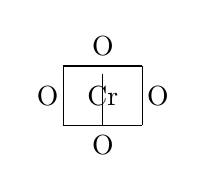
\begin{tikzpicture}[scale=0.5]
  \draw (0,0) -- (2,0);
  \draw (0,0) -- (0,-1.5);
  \draw (2,0) -- (2,-1.5);
  \draw (1,-0.2) -- (1,-1.5);
  \draw (0,-1.5) -- (2,-1.5);
  \node at (1,0.5) {O};
  \node at (-0.4,-0.75) {O};
  \node at (2.4,-0.75) {O};
  \node at (1,-2) {O};
  \node at (1,-0.75) {Cr};
\end{tikzpicture}
\end{center}
\begin{options}
  \item $+10$
  \item $+6$
  \item $+3$
  \item $+2$
\end{options}

\item The oxidation state of Fe in \ce{Fe3O4} is
\begin{options}
  \item $+3$
  \item $+8/3$
  \item $+6$
  \item $+2$
\end{options}

\item The oxidation number of oxygen in \ce{KO3} and \ce{Na2O2} respectively is
\begin{options}
  \item 3, 2
  \item 1, 0
  \item 0, 1
  \item $-0.33, -1$
\end{options}

\item What is the oxidation state of P in \ce{Ba(H2PO2)2}?
\begin{options}
  \item $+1$
  \item $+2$
  \item $+3$
  \item $-1$
\end{options}

\item The oxidation number of Cr in \ce{K2CrO4} is
\begin{options}
  \item $+3$
  \item $-6$
  \item $+6$
  \item $-3$
\end{options}

\item Oxidation number of sulphur in Caro's acid is
\begin{options}
  \item $+6$
  \item $+4$
  \item $+8$
  \item $+7$
\end{options}

\item What is the oxidation number of chlorine in \ce{ClO3-}?
\begin{options}
  \item $+5$
  \item $+3$
  \item $+4$
  \item $+2$
\end{options}

\item Arrange the following as in increase in oxidation number.\\
(i) \ce{Mn^{2+}} \quad (ii) \ce{MnO2} \quad (iii) \ce{KMnO4} \quad (iv) \ce{K2MnO4}
\begin{options}
  \item (i) $>$ (ii) $>$ (iii) $>$ (iv)
  \item (i) $<$ (ii) $<$ (iv) $<$ (iii)
  \item (ii) $<$ (iii) $<$ (i) $<$ (iv)
  \item (iii) $>$ (i) $>$ (iv) $>$ (ii)
\end{options}

\item Nitrogen has fractional oxidation number in:
\begin{options}
  \item \ce{N2H4}
  \item \ce{NH4}
  \item \ce{N2H}
  \item \ce{N2F3}
\end{options}

\item Oxidation state of carbon in graphite is:
\begin{options}
  \item Zero
  \item $+1$
  \item $+4$
  \item $+2$
\end{options}

\item Oxidation number of S in \ce{(CH3)2SO} is:
\begin{options}
  \item Zero
  \item $+1$
  \item $+2$
  \item $+3$
\end{options}

\item Oxidation number of nitrogen in \ce{AgNO3} is:
\begin{options}
  \item $+5$
  \item $-3$
  \item $+3$
  \item $-2$
\end{options}

\item Oxidation number of Fe in \ce{K3[Fe(CN)6]} is:
\begin{options}
  \item $+2$
  \item $+3$
  \item $+4$
  \item $+1$
\end{options}

\item The oxidation number of iodine in \ce{IF5} is:
\begin{options}
  \item $+5$
  \item $-5$
  \item $-1$
  \item $+1$
\end{options}

\item The oxidation state of nitrogen in \ce{NH4NO3} is:
\begin{options}
  \item $-3$ and $+5$
  \item $+3$ and $+5$
  \item $+5$
  \item $+3$
\end{options}

\item Oxidation state of oxygen atom in potassium superoxide (\ce{KO2}) is:
\begin{options}
  \item $-1/2$
  \item Zero
  \item $+1/2$
  \item $-2$
\end{options}

\item Which of the following shows highest oxidation no. in combined state?
\begin{options}
  \item Os
  \item Ru
  \item Both (1) and (2)
  \item Mn
\end{options}

\item The oxidation number of carbon in \ce{H2C2O4} is:
\begin{options}
  \item $+2$
  \item $+3$
  \item $+4$
  \item $+1$
\end{options}

\item The oxidation state of nitrogen varies from:
\begin{options}
  \item $-3$ to $+5$
  \item $0$ to $+5$
  \item $-3$ to $1$
  \item $+3$ to $+5$
\end{options}

\item Iodine has $+7$ oxidation state in:
\begin{options}
  \item \ce{HIO4}
  \item \ce{H3IO5}
  \item \ce{H5IO6}
  \item All of these
\end{options}

\item The oxidation number of Cr in \ce{[Cr(NH3)4Cl2]+} is:
\begin{options}
  \item $+3$
  \item $+2$
  \item $+1$
  \item zero
\end{options}

\item In the compounds \ce{KMnO4} and \ce{K2Cr2O7}, the highest oxidation state is of the element
\begin{options}
  \item Mn
  \item K
  \item O
  \item Cr
\end{options}

\item When \ce{K2Cr2O7} is converted into \ce{K2CrO4}, the change in oxidation number of chromium is
\begin{options}
  \item 0
  \item 5
  \item 7
  \item 9
\end{options}

\item In the conversion of \ce{Br2} to \ce{BrO3-}, the oxidation number of Br changes from
\begin{options}
  \item Zero to $+5$
  \item $+1$ to $+5$
  \item Zero to 3
  \item $+2$ to $+5$
\end{options}

\item Oxidation state of oxygen in \ce{H2O2} is
\begin{options}
  \item $-1$
  \item $+2$
  \item $+1/2$
  \item $-2$
\end{options}

\item In the equation, \ce{CrO4^{2-} + SO3^{2-} -> Cr(OH)4- + SO4^{2-}} the oxidation number of Cr changes from
\begin{options}
  \item 6 to 4
  \item 6 to 3
  \item 8 to 4
  \item 4 to 3
\end{options}

\item Manganese acts as strongest oxidising agent in the oxidation state
\begin{options}
  \item $+7$
  \item $+2$
  \item $+4$
  \item $+5$
\end{options}

\item The difference in the oxidation numbers of the two types of sulphur atoms in \ce{Na2S4O6} is
\begin{options}
  \item 4
  \item 5
  \item 6
  \item 7
\end{options}

\item The oxidation number of N and Cl in \ce{NOClO4} respectively are
\begin{options}
  \item $+2$ and $+7$
  \item $+3$ and $+7$
  \item $-3$ and $+5$
  \item $+2$ and $-7$
\end{options}

\item Oxidation number of P in \ce{HP2O7-} ion is
\begin{options}
  \item $+5$
  \item $+6$
  \item $+7$
  \item $+3$
\end{options}

\item What is the oxidation no. of Mn in \ce{K2MnO4}?
\begin{options}
  \item $+4$
  \item $+6$
  \item $+2$
  \item $+8$
\end{options}

\item The oxidation state of chlorine is highest in the compound:
\begin{options}
  \item \ce{Cl2}
  \item HCl
  \item \ce{ClO}
  \item \ce{Cl2O7}
\end{options}

\item The oxidation number that iron does not exhibit in its common compounds or in its elemental state is:
\begin{options}
  \item Zero
  \item $+1$
  \item $+2$
  \item $+3$
\end{options}

\item Maximum oxidation state is present in:
\begin{options}
  \item \ce{CrO2Cl2} and \ce{MnO4-}
  \item \ce{MnO2}
  \item \ce{[Fe(CN)6]^{3-}} and \ce{[Co(CN)6]^{3-}}
  \item MnO
\end{options}

\item In the reaction, \ce{2Na2S2O3 + I2 -> Na2S4O6 + 2NaI}, the oxidation state of sulphur is:
\begin{options}
  \item Decreased
  \item Increased
  \item Unchanged
  \item None of these
\end{options}

\item The oxidation state of two sulphur atoms in \ce{H2S2O8}
\begin{options}
  \item $-6$
  \item $-2$
  \item $+6$
  \item $-4$
\end{options}

\item Oxidation state of sulphur in \ce{Na2S2O3} and \ce{Na2S4O6}
\begin{options}
  \item 4 and 6
  \item 3 and 5
  \item 2 and 2.5
  \item 6 and 6
\end{options}

\item Sulphur in $+3$ oxidation state is present in
\begin{options}
  \item Sulphurous acid
  \item Pyrosulphuric acid
  \item Dithionous acid
  \item Thiosulphuric acid
\end{options}

\item When sulphur dioxide is passed in an acidified \ce{K2Cr2O7} solution, the oxidation state of sulphur is changed from
\begin{options}
  \item 4 to 0
  \item 4 to 2
  \item 4 to 6
  \item 6 to 4
\end{options}

\item In which of the following, oxygen shows $-1$ oxidation state?
\begin{options}
  \item \ce{H2O2}
  \item \ce{CO2}
  \item \ce{H2O}
  \item \ce{OF2}
\end{options}

\item In which of the following, the oxidation number of oxygen has been arranged in increasing order?
\begin{options}
  \item \ce{OF2} $<$ \ce{KO2} $<$ \ce{BaO2} $<$ \ce{O3}
  \item \ce{BaO2} $<$ \ce{KO2} $<$ \ce{O3} $<$ \ce{OF2}
  \item \ce{BaO2} $<$ \ce{O3} $<$ \ce{OF2} $<$ \ce{KO2}
  \item \ce{KO2} $<$ \ce{O3} $<$ \ce{BaO2} $<$ \ce{OF2}
\end{options}

\item As the oxidation state for any metal increases, the tendency to show ionic nature:
\begin{options}
  \item Decreases
  \item Increases
  \item Remains same
  \item None of these
\end{options}

\item The most stable oxidation state of chromium is:
\begin{options}
  \item $+5$
  \item $+3$
  \item $+2$
  \item $+4$
\end{options}

\end{questions}
\end{multicols}

% ============================================================
\begin{mdframed}[backgroundcolor=sectionbg, linewidth=0pt, innerleftmargin=6pt, innerrightmargin=6pt, innertopmargin=4pt, innerbottommargin=4pt]
\color{white}\bfseries\small\centering BALANCING OF REDOX REACTIONS
\end{mdframed}

\begin{multicols}{2}
\begin{questions}[start=107]

\item Reaction of \ce{Br2} with \ce{Na2CO3} in aqueous solution gives sodium bromide and sodium bromate with evolution of \ce{CO2} gas. The number of sodium bromide molecules involved in the balanced chemical equation is
\begin{options}
  \item 1
  \item 3
  \item 5
  \item 7
\end{options}

\item \ce{aK2Cr2O7 + bKCl + cH2SO4 -> xClO2Cl2 + yKHSO4 + zH2O}.\\
The above equation balances when
\begin{options}
  \item $a=2, b=4, c=6$ and $x=2, y=6, z=3$
  \item $a=4, b=2, c=6$ and $x=6, y=2, z=3$
  \item $a=6, b=4, c=2$ and $x=6, y=3, z=2$
  \item $a=1, b=4, c=6$ and $x=2, y=6, z=3$
\end{options}

\item In the ionic equation, \ce{BiO3- + 6H+ + xe- -> Bi^{3+} + 3H2O}. The value of $x$ is
\begin{options}
  \item 6
  \item 2
  \item 4
  \item 3
\end{options}

\item For the reaction, \ce{NH3 + OCl- -> N2H4 + Cl-} occurring in basic medium, the coefficient of \ce{N2H4} in the balanced equation will be
\begin{options}[start=1]
  \item 1
  \item 2
  \item 3
  \item 4
\end{options}

\item The value of `$n$' in the reaction\\
\ce{Cr2O7^{2-} + 14H+ + nFe^{2+} -> 2Cr^{3+} + nFe^{3+} + 7H2O} will be
\begin{options}
  \item 2
  \item 3
  \item 6
  \item 7
\end{options}

\item The number of moles of \ce{KMnO4} reduced by one mole of KI in alkaline medium is
\begin{options}
  \item 1
  \item 5
  \item 1/2
  \item 1/5
\end{options}

\item The value of $n$ in \ce{MnO4- + 8H+ + ne- -> Mn^{2+} + 4H2O} is
\begin{options}
  \item 5
  \item 4
  \item 2
  \item 3
\end{options}

\item In the reactions; \ce{As2S3 + HNO3 -> H3AsO4 + H2SO4 + NO}, the element oxidized is/are:
\begin{options}
  \item As only
  \item S only
  \item N only
  \item As and S both
\end{options}

\item In balancing the half reaction, \ce{S2O3^{2-} -> S(s)}, the number of electrons that must be added is:
\begin{options}
  \item 2 on the right
  \item 2 on the left
  \item 3 on the right
  \item 4 on the left
\end{options}

\item What volume of 3 molar \ce{HNO3} is needed to oxidise 8 g of \ce{Fe^{2+}} to \ce{Fe^{3+}}? \ce{HNO3} gets converted to NO:
\begin{options}
  \item 8 mL
  \item 16 mL
  \item 32 mL
  \item 64 mL
\end{options}

\item In the reduction of dichromate by Fe (II), the number of electrons involved per chromium atom is:
\begin{options}
  \item 3
  \item 1
  \item 2
  \item 4
\end{options}

\item In the following reaction\\
\ce{M^{x+} + MnO4- -> MO3- + Mn^{2+} + \frac{1}{2}O2}\\
If one mole of \ce{MnO4-} oxidises 2.5 moles of \ce{M^{x+}} then the value of $x$ is
\begin{options}
  \item 5
  \item 3
  \item 4
  \item 2
\end{options}

\end{questions}
\end{multicols}

% ============================================================
\begin{mdframed}[backgroundcolor=sectionbg, linewidth=0pt, innerleftmargin=6pt, innerrightmargin=6pt, innertopmargin=4pt, innerbottommargin=4pt]
\color{white}\bfseries\small\centering REDOX REACTIONS AS THE BASIS FOR TITRATIONS
\end{mdframed}

\begin{multicols}{2}
\begin{questions}[start=119]

\item During a redox titration involving a solution containing \ce{Fe^{2+}} ions against \ce{MnO4-} in the presence of excess of \ce{H+} ions, the number of electrons that gets transferred is
\begin{options}
  \item 6
  \item 5
  \item 4
  \item 2
\end{options}

\item Which one of the compound does not decolourised an acidified solution of \ce{KMnO4}?
\begin{options}
  \item \ce{SO2}
  \item \ce{FeCl3}
  \item \ce{H2O2}
  \item \ce{FeSO4}
\end{options}

\item How many moles of electron are involved in the reduction of one mole of \ce{MnO4-} ion in alkaline medium to \ce{MnO3-}?
\begin{options}
  \item 2
  \item 1
  \item 3
  \item 4
\end{options}

\item If \ce{H2S} is passed through an acidified \ce{K2Cr2O7} solution, the colour of the solution:
\begin{options}
  \item Will remain unchanged
  \item Will change to deep red
  \item Will change to dark green
  \item Will change to dark brown
\end{options}

\item When an acidified solution of ferrous ammonium sulphate is treated with \ce{KMnO4} solution, the ion which is oxidised is:
\begin{options}
  \item \ce{Fe^{2+}}
  \item \ce{SO4^{2-}}
  \item \ce{NH4+}
  \item \ce{MnO4-}
\end{options}

\item Reaction of acidified \ce{KMnO4} with ferrous oxalate gives oxidation products containing:
\begin{options}
  \item \ce{Fe^{3+}}
  \item \ce{CO2}
  \item Both (1) and (2)
  \item \ce{Fe^{2+}}
\end{options}

\item In presence of dil. \ce{H2SO4}, the equivalent weight of \ce{KMnO4} is
\begin{options}
  \item 1/5 of its molecular weight
  \item 1/6 of its molecular weight
  \item 1/10 of its molecular weight
  \item 1/2 of its molecular weight
\end{options}

\item In the reaction, \ce{2CuSO4 + 4KI -> Cu2I2 + 2K2SO4 + I2}. The ratio of equivalent weight of \ce{CuSO4} to its molecular weight is:
\begin{options}
  \item 1/8
  \item 1/4
  \item 1/2
  \item 1
\end{options}

\item In the reaction, \ce{N2 -> NH3}. The eq.wt. of \ce{N2} and \ce{NH3} are respectively equal to:
\begin{options}
  \item $\frac{28}{3}, \frac{17}{3}$
  \item $\frac{28}{6}, \frac{17}{3}$
  \item $\frac{28}{2}, \frac{17}{2}$
  \item $\frac{28}{5}, \frac{17}{5}$
\end{options}

\item The equivalent weight of \ce{KMnO4} (acidic medium) is (at. wt. of K = 39; Mn = 55):
\begin{options}
  \item 158
  \item 15.8
  \item 31.6
  \item 3.16
\end{options}

\item The equivalent weight of iron in \ce{Fe2O3} would be:
\begin{options}
  \item 18.6
  \item 28
  \item 56
  \item 11
\end{options}

\item In alkaline condition \ce{KMnO4} reacts as follows,\\
\ce{2KMnO4 + 2KOH -> 2K2MnO4 + H2O + O}\\
Therefore, its equivalent weight will be:
\begin{options}
  \item 31.6
  \item 52.7
  \item 79.0
  \item 158.0
\end{options}

\item 1 mole of \ce{MnO4^{2-}} in neutral aqueous medium disproportionates to:
\begin{options}
  \item $\frac{2}{3}$ mole of \ce{MnO4} and $\frac{1}{3}$ mole of \ce{MnO2}
  \item $\frac{1}{3}$ mole of \ce{MnO4} and $\frac{2}{3}$ mole of \ce{MnO2}
  \item $\frac{1}{3}$ mole of $\frac{1}{3}$ and mole of \ce{MnO2}
  \item $\frac{2}{3}$ mole of \ce{Mn2O7} and $\frac{1}{3}$ mole of \ce{MnO2}
\end{options}

\item Titre value is the volume of titrant used for a definite amount of unknown reagent at its
\begin{options}
  \item Equivalence point
  \item End point
  \item Neutralization point
  \item All of these
\end{options}

\item When \ce{BrO3-} ion reacts with \ce{Br-} ion in acidic solution \ce{Br2} is liberated. The equivalent weight of \ce{KBrO3} is:
\begin{options}
  \item M/8
  \item M/3
  \item M/5
  \item M/6
\end{options}

\item The eq. wt. of \ce{K2CrO4} as an oxidising agent in acid medium is:
\begin{options}
  \item (mol. wt.)/2
  \item (2 $\times$ mol. wt.)/3
  \item (mol. wt.)/3
  \item (mol. wt.)/6
\end{options}

\item Which one is not a redox titration?
\begin{options}
  \item \ce{FeSO4} vs. \ce{K2Cr2O7}
  \item \ce{CuSO4} vs. hypo
  \item \ce{I2} vs. hypo
  \item \ce{AgNO3} vs. KCl
\end{options}

\item Starch gives blue colour with
\begin{options}
  \item KI
  \item \ce{I2}
  \item \ce{Cl2}
  \item None of these
\end{options}

\item Equivalent mass of \ce{Na2S2O3} in its reaction with \ce{I2} is equal to:
\begin{options}
  \item Molar mass
  \item Molar mass/2
  \item Molar mass/3
  \item Molar mass/4
\end{options}

\end{questions}
\end{multicols}

% ============================================================
\begin{mdframed}[backgroundcolor=sectionbg, linewidth=0pt, innerleftmargin=6pt, innerrightmargin=6pt, innertopmargin=4pt, innerbottommargin=4pt]
\color{white}\bfseries\small\centering REDOX REACTIONS AND ELECTRODE PROCESS
\end{mdframed}

\begin{multicols}{2}
\begin{questions}[start=138]

\item Which one of the following reaction is possible at anode?
\begin{options}
  \item \ce{F2 + 2e- -> 2F-}
  \item \ce{2H+ + \frac{1}{2}O2 + 2e- -> H2O}
  \item \ce{2Cr^{3+} + 7H2O -> Cr2O7^{2-} + 14H+ + 6e-}
  \item \ce{Fe^{2+} -> Fe^{3+} + e-}
\end{options}

\item When Fe metal is rusted then Fe is:
\begin{options}
  \item Oxidised
  \item Reduced
  \item Hydrolysed
  \item Precipitated
\end{options}

\item The function of a salt bridge is to
\begin{options}
  \item eliminate the impurities present in the electrolyte
  \item eliminate liquid-junction potential where the ions are present in excess at the junction
  \item decrease the cell potential at the negative electrode
  \item increase the cell potential at the positive electrode
\end{options}

\item Reduction potential of $A$, $B$, $C$ and $D$ are 0.8 V, 0.79 V, 0.34 V and $-2.37$ V respectively. Which element displaces all other three elements?
\begin{options}
  \item B
  \item A
  \item D
  \item C
\end{options}

\item a. \ce{Fe^{3+} + e- -> Fe^{2+}aq} \quad $E^o = +0.77$ V\\
b. \ce{Al^{3+} + 3e- -> Al(s)} \quad $E^o = -1.66$ V\\
c. \ce{Br2 + 2e- -> 2Br-aq} \quad $E^o = +1.08$ V\\
Based on the data given above, the correct order of reducing power is
\begin{options}
  \item \ce{Br2} $<$ \ce{Fe^{3+}} $<$ Al
  \item \ce{Br-} $<$ \ce{Fe^{2+}} $<$ Al
  \item \ce{Fe^{2+}} $<$ Al $<$ \ce{Br-}
  \item Al $<$ \ce{Br-} $<$ \ce{Fe^{2+}}
\end{options}

\end{questions}
\end{multicols}

% ============================================================
\begin{mdframed}[backgroundcolor=sectionbg, linewidth=0pt, innerleftmargin=6pt, innerrightmargin=6pt, innertopmargin=4pt, innerbottommargin=4pt]
\color{white}\bfseries\small\centering MIXED CONCEPT QUESTIONS
\end{mdframed}

\begin{multicols}{2}
\begin{questions}[start=1]

\item \ce{H2O2} reduces \ce{MnO4-} ion to
\begin{options}
  \item \ce{Mn+}
  \item \ce{Mn^{2+}}
  \item \ce{Mn^{3+}}
  \item \ce{Mn-}
\end{options}

\item When a sulphur atom becomes a sulphide ion
\begin{options}
  \item There is no change in the composition of atom
  \item It gains two electrons
  \item The mass number changes
  \item The atomic number changes
\end{options}

\item The ultimate products of oxidation of most of hydrogen and carbon in food stuffs are
\begin{options}
  \item \ce{H2O} alone
  \item \ce{CO2} alone
  \item \ce{H2O} and \ce{CO2}
  \item \ce{H2O} and CO
\end{options}

\item In the reaction \ce{H2S + NO2 -> H2O + NO + S}. \ce{H2S} is
\begin{options}
  \item Oxidised
  \item Reduced
  \item Precipitated
  \item Neither oxidized nor reduced
\end{options}

\item The conversion of \ce{PbO2} to \ce{Pb(NO3)2} is
\begin{options}
  \item Oxidation
  \item Reduction
  \item Neither oxidation nor reduction
  \item Both oxidation and reduction
\end{options}

\item In the course of a chemical reaction, an oxidant
\begin{options}
  \item Loses electrons
  \item Gains electrons
  \item Both loses and gains electron
  \item Electron change takes place
\end{options}

\item \ce{2CuI -> Cu + CuI2}, the reaction is
\begin{options}
  \item Redox
  \item Neutralisation
  \item Oxidation
  \item Reduction
\end{options}

\item \ce{H2O2} reduces \ce{K4Fe(CN)6}
\begin{options}
  \item In neutral solution
  \item In acidic solution
  \item In non-polar solvent
  \item In alkaline solution
\end{options}

\item In the reaction \ce{3Mg + N2 -> Mg3N2}
\begin{options}
  \item Magnesium is reduced
  \item Magnesium is oxidized
  \item Nitrogen is oxidized
  \item Both magnesium and nitrogen are reduced
\end{options}

\item When sodium metal is dissolved in liquid ammonia, blue colour solution is formed. The blue colour is due to
\begin{options}
  \item Solvated \ce{Na+} ions
  \item Solvated electrons
  \item Solvated \ce{NH2-} ions
  \item Solvated protons
\end{options}

\item Following reaction describes the rusting of iron\\
\ce{4Fe + 3O2 -> 4Fe^{3+} + 6O^{2-}}\\
Which one of the following statement is incorrect?
\begin{options}
  \item This is an example of a redox reaction
  \item Metallic iron is reduced to \ce{Fe^{3+}}
  \item \ce{Fe^{3+}} is an oxidising agent
  \item Metallic iron is a reducing agent
\end{options}

\item \ce{SnCl2} gives a precipitate with a solution of \ce{HgCl2}. In this process, \ce{HgCl2} is
\begin{options}
  \item Reduced
  \item Oxidised
  \item Converted into a complex compound containing both Sn and Hg
  \item Converted into a chloro complex of Hg
\end{options}

\item Oxidation involves
\begin{options}
  \item Loss of electrons
  \item Gain of electrons
  \item Increase in the valency of negative part
  \item Decrease in the valency of positive part
\end{options}

\item Incorrect statement regarding rusting is
\begin{options}
  \item Metallic iron is oxidised to \ce{Fe^{3+}} ions
  \item Metallic iron is reduced to \ce{Fe^{2-}} ions
  \item Oxygen gas is reduced to oxide ion
  \item Yellowish -- brown product is formed
\end{options}

\item When copper turnings are added to silver nitrate solution, a blue coloured solution is formed after some time. It is because, copper
\begin{options}
  \item Displaces silver from the solution
  \item Forms a blue coloured complex with \ce{AgNO3}
  \item Is oxidised to \ce{Cu^{2+}}
  \item Is reduced to \ce{Cu^{2+}}
\end{options}

\item Equation \ce{H2S + H2O2 -> S + 2H2O} represents
\begin{options}
  \item Acidic nature of \ce{H2O2}
  \item Basic nature of \ce{H2O2}
  \item Oxidising nature of \ce{H2O2}
  \item Reducing nature of \ce{H2O2}
\end{options}

\item In the reaction\\
\ce{C2O4^{2-} + MnO4- + H+ -> Mn^{2+} + CO2 + H2O}\\
the reductant is
\begin{options}
  \item \ce{C2O4^{2-}}
  \item \ce{MnO4-}
  \item \ce{Mn^{2+}}
  \item \ce{H+}
\end{options}

\item Which of the following is the most powerful oxidizing agent?
\begin{options}
  \item \ce{F2}
  \item \ce{Cl2}
  \item \ce{Br2}
  \item \ce{I2}
\end{options}

\item Of the four oxyacids of chlorine, the strongest oxidising agent in dilute aqueous solution is
\begin{options}
  \item \ce{HClO4}
  \item \ce{HClO3}
  \item \ce{HClO4}
  \item HOCl
\end{options}

\item Identify the correct statement about \ce{H2O2}
\begin{options}
  \item It acts as reducing agent only.
  \item It acts as both oxidising and reducing agent.
  \item It is neither an oxidiser nor reducer.
  \item It acts as oxidising agent only.
\end{options}

\item Several blocks of magnesium are fixed to the bottom of a ship to
\begin{options}
  \item Keep away the sharks
  \item Make the ship lighter
  \item Prevent action of water and salt
  \item Prevent puncturing by under-sea rocks
\end{options}

\item Which of the following behaves as both oxidising and reducing agents?
\begin{options}
  \item \ce{H2SO4}
  \item \ce{SO2}
  \item \ce{H2S}
  \item \ce{HNO3}
\end{options}

\item Which of the following is not a reducing agent?
\begin{options}
  \item \ce{NaNO2}
  \item \ce{NaNO3}
  \item HI
  \item \ce{SnCl2}
\end{options}

\item Which of the following cannot work as oxidising agent?
\begin{options}
  \item \ce{O2}
  \item \ce{KMnO4}
  \item \ce{I2}
  \item None of these
\end{options}

\item In \ce{C + H2O -> CO + H2}, \ce{H2O} acts as
\begin{options}
  \item Oxidising agent
  \item Reducing agent
  \item (1) and (2) both
  \item Neither (1) nor (2)
\end{options}

\item Strongest reducing agent is
\begin{options}
  \item \ce{F-}
  \item \ce{Cl-}
  \item \ce{Br-}
  \item \ce{I-}
\end{options}

\item A solution of sulphur dioxide in water reacts with \ce{H2S} precipitating sulphur. Here, sulphur dioxide acts as
\begin{options}
  \item As oxidising agent
  \item A reducing agent
  \item An acid
  \item A catalyst
\end{options}

\item Which of these substances is a good reducing agent?
\begin{options}
  \item NaOCl
  \item HI
  \item \ce{FeCl3}
  \item KBr
\end{options}

\item The strongest reducing agent is
\begin{options}
  \item \ce{HNO2}
  \item \ce{H2S}
  \item \ce{H2SO3}
  \item \ce{SnCl2}
\end{options}

\item Which one is an oxidising agent?
\begin{options}
  \item \ce{FeSO4}
  \item \ce{HNO3}
  \item \ce{FeSO4.(NH4)2SO4.6H2O}
  \item \ce{H2S}
\end{options}

\item In which of the following reactions, \ce{H2O2} is a reducing agent?
\begin{options}
  \item \ce{2FeCl2 + 2HCl + H2O2 -> 2FeCl3 + 2H2O}
  \item \ce{Cl2 + H2O2 -> 2HCl + O2}
  \item \ce{2HI + H2O2 -> 2H2O + I2}
  \item \ce{H2SO3 + H2O2 -> H2SO4 + H2O}
\end{options}

\item When NaCl is dissolved in water, the sodium ion is
\begin{options}
  \item Oxidised
  \item Reduced
  \item Hydrolysed
  \item Hydrated
\end{options}

\item Strongest reducing agent is
\begin{options}
  \item K
  \item Mg
  \item Al
  \item Br
\end{options}

\item Which substance is serving as a reducing agent in the following reaction?\\
\ce{14H+ + Cr2O7^{2-} + 3Ni -> 2Cr^{3+} + 7H2O + 3Ni^{2+}}
\begin{options}
  \item \ce{H2O}
  \item Ni
  \item \ce{H+}
  \item \ce{Cr2O7^{2-}}
\end{options}

\item Which of the following acid possesses oxidising, reducing and complex forming properties?
\begin{options}
  \item \ce{HNO3}
  \item \ce{H2SO4}
  \item HCl
  \item \ce{HNO2}
\end{options}

\item Which one is an oxidising substance?
\begin{options}
  \item \ce{C2H2O2}
  \item CO
  \item \ce{H2S}
  \item \ce{CO2}
\end{options}

\item The compound that can work both as oxidising and reducing agent is
\begin{options}
  \item \ce{KMnO4}
  \item \ce{H2O2}
  \item \ce{BaO2}
  \item \ce{K2Cr2O7}
\end{options}

\item The oxidation number of C in \ce{CO2} is
\begin{options}
  \item $-2$
  \item $+2$
  \item $-4$
  \item $+4$
\end{options}

\item The oxidation number of As is
\begin{options}
  \item $+2$ and $3$
  \item $+3$ and $+5$
  \item $+3$ and $+4$
  \item $+1$ and $+2$
\end{options}

\item The oxidation number of Ba in barium peroxide is
\begin{options}
  \item $+6$
  \item $+2$
  \item $+1$
  \item $+4$
\end{options}

\item \ce{HNO2} acts both as reductant and oxidant, while \ce{HNO3} acts only as oxidant. It is due to their
\begin{options}
  \item Solubility
  \item Maximum oxidation number
  \item Minimum oxidation number
  \item Minimum number of valence electrons
\end{options}

\item Chlorine is in $+1$ oxidation state in
\begin{options}
  \item HCl
  \item \ce{HClO4}
  \item ICl
  \item \ce{Cl2O}
\end{options}

\item The valency of Cr in the complex \ce{[Cr(H2O)4Cl2]+}
\begin{options}
  \item 1
  \item 3
  \item 5
  \item 6
\end{options}

\item In the conversion \ce{Br2 -> BrO3-}, the oxidation state of bromine changes from
\begin{options}
  \item $-1$ to $-1$
  \item $0$ to $-1$
  \item $0$ to $+5$
  \item $0$ to $-5$
\end{options}

\item In the chemical reaction \ce{Cl2 + H2S -> 2HCl + S}, the oxidation number of sulphur changes from
\begin{options}
  \item 0 to 2
  \item 2 to 0
  \item $-2$ to 0
  \item $-2$ to $-1$
\end{options}

\item Oxidation number of cobalt in \ce{K[Co(CO)4]} is
\begin{options}
  \item $+1$
  \item $+3$
  \item $-1$
  \item $-3$
\end{options}

\item When \ce{K2Cr2O7} is converted to \ce{K2CrO4}, the change in the oxidation state of chromium is
\begin{options}
  \item 0
  \item 6
  \item 4
  \item 3
\end{options}

\item The oxidation number of chlorine in HOCl
\begin{options}
  \item $-1$
  \item 0
  \item $+1$
  \item $+2$
\end{options}

\item Oxidation number of S in \ce{S^{2-}} is
\begin{options}
  \item $-2$
  \item 0
  \item $-6$
  \item $+2$
\end{options}

\item Oxidation number of N in \ce{(NH4)2SO4} is
\begin{options}
  \item $-1/3$
  \item $-1$
  \item $+1$
  \item $-3$
\end{options}

\item In which compound, oxidation state of nitrogen is $+1$?
\begin{options}
  \item NO
  \item \ce{N2O}
  \item \ce{NH2OH}
  \item \ce{N2H4}
\end{options}

\item Oxidation number of nickel in \ce{Ni(CO)4}
\begin{options}
  \item 0
  \item $+2$
  \item $-4$
  \item $+2$
\end{options}

\item The oxidation number of sulphur in \ce{H2SO4} is
\begin{options}
  \item $-2$
  \item $+2$
  \item $+4$
  \item $+6$
\end{options}

\item Oxidation state of chlorine in perchloric acid is
\begin{options}
  \item $-1$
  \item 0
  \item $-7$
  \item $+7$
\end{options}

\item Oxidation number of N in \ce{HNO3} is
\begin{options}
  \item $-3.5$
  \item $+3.5$
  \item $-3, +5$
  \item $+5$
\end{options}

\item The oxidation number of Mn in \ce{MnO4-} is
\begin{options}
  \item $+7$
  \item $-5$
  \item $+6$
  \item $+5$
\end{options}

\item \ce{Sn^{n+}} loses two electrons in a reaction. What will be the oxidation number of tin after the reaction
\begin{options}
  \item $+2$
  \item Zero
  \item $+4$
  \item $-2$
\end{options}

\item The oxidation state of Mn in \ce{K2MnO4}
\begin{options}
  \item $+2$
  \item $+7$
  \item $-2$
  \item $+6$
\end{options}

\item Oxidation number of oxygen in \ce{O2} molecule is
\begin{options}
  \item $+1$
  \item 0
  \item $+2$
  \item $-2$
\end{options}

\item Maximum oxidation state of Cr is
\begin{options}
  \item $+3$
  \item $+4$
  \item $+6$
  \item $+7$
\end{options}

\item In which of the following compounds transition metal has zero oxidation state
\begin{options}
  \item \ce{CrO5}
  \item \ce{K2Cr2O7}
  \item \ce{MnO2}
  \item \ce{[Fe(CO)5]}
\end{options}

\item Carbon is in the lowest oxidation state in
\begin{options}
  \item \ce{CH4}
  \item \ce{CCl4}
  \item \ce{CF4}
  \item \ce{CO2}
\end{options}

\item Oxidation number of carbon in \ce{H2C2O4} is
\begin{options}
  \item $+4$
  \item $+3$
  \item $+2$
  \item $-2$
\end{options}

\item The oxidation number of Pt in \ce{[Pt(C2H4)Cl3]-} is
\begin{options}
  \item $+1$
  \item $+2$
  \item $+3$
  \item $+4$
\end{options}

\item The oxidation number of carbon in \ce{CH2Cl2} is
\begin{options}
  \item 0
  \item $+2$
  \item $-2$
  \item $+4$
\end{options}

\item The oxidation states of phosphorus vary from
\begin{options}
  \item $-3$ to $+5$
  \item $-1$ to $+1$
  \item $-3$ to $+3$
  \item $-5$ to $+1$
\end{options}

\item The process in which oxidation number increases is known as
\begin{options}
  \item Oxidation
  \item Reduction
  \item Auto-oxidation
  \item Decomposition
\end{options}

\item The oxidation number of S in \ce{H2S2O8} is
\begin{options}
  \item $+2$
  \item $+4$
  \item $+6$
  \item $+7$
\end{options}

\item The oxidation state of nitrogen in \ce{N3H} is
\begin{options}
  \item $+1/3$
  \item $+3$
  \item $-1$
  \item $-1/3$
\end{options}

\item Which of the following statements is correct?
\begin{options}
  \item Hydrogen has oxidation number $-1$ and $+1$.
  \item Hydrogen has same electronegativity as halogens.
  \item Hydrogen will not be liberated at anode.
  \item Hydrogen has same ionization potential as alkali metals.
\end{options}

\item The oxidation state of Cr in \ce{[Cr(NH3)4Cl2]+} is
\begin{options}
  \item $+3$
  \item $+2$
  \item $+1$
  \item 0
\end{options}

\item Sulphur has highest oxidation state in
\begin{options}
  \item \ce{SO2}
  \item \ce{H2SO4}
  \item \ce{Na2S2O3}
  \item \ce{Na2S4O6}
\end{options}

\item The oxidation number of Fe and S in iron pyrites are
\begin{options}
  \item $+4, -2$
  \item $+2, -1$
  \item $+3, -1.5$
  \item $+3, -1$
\end{options}

\item The oxidation number of nitrogen in \ce{NO3-} is
\begin{options}
  \item $-1$
  \item $+2$
  \item $+3$
  \item $+5$
\end{options}

\item Oxidation state of elemental carbon is
\begin{options}
  \item 0
  \item 1
  \item 2
  \item 3
\end{options}

\item Which one of the following has the highest oxidation number of iodine?
\begin{options}
  \item \ce{KI3}
  \item KI
  \item \ce{IF5}
  \item \ce{KIO4}
\end{options}

\item The oxidation number of N in \ce{N2H4+}
\begin{options}
  \item $-3$
  \item $(-2)$
  \item $-1$
  \item $+2$
\end{options}

\item In which of the following compounds, the oxidation number of carbon is maximum?
\begin{options}
  \item HCHO
  \item \ce{CHCl3}
  \item \ce{CH3OH}
  \item \ce{C12H22O11}
\end{options}

\item The oxidation state of chlorine in \ce{KClO4} is
\begin{options}
  \item $-1$
  \item $+1$
  \item $+7$
  \item $-7$
\end{options}

\item The oxidation state of I in \ce{H4IO6-} is
\begin{options}
  \item $+7$
  \item $+5$
  \item $+3$
  \item $-1$
\end{options}

\item An element which never has a positive oxidation number in any of its compounds
\begin{options}
  \item Boron
  \item Oxygen
  \item Chlorine
  \item Fluorine
\end{options}

\item In an oxidation process, oxidation number
\begin{options}
  \item Decreases
  \item Increases
  \item Does not change
  \item First increases then decreases
\end{options}

\item If \ce{HNO3} changes into \ce{N2O}, the oxidation number is changed by
\begin{options}
  \item $+2$
  \item $-1$
  \item 0
  \item $+4$
\end{options}

\item The characteristic oxidation number of atoms in free metals is
\begin{options}
  \item Minus one
  \item Any number
  \item One
  \item Zero
\end{options}

\item In which one of the following changes, there are transfer of five electrons?
\begin{options}
  \item \ce{MnO4- -> Mn^{2+}}
  \item \ce{CrO4^{2-} -> Cr^{3+}}
  \item \ce{MnO4^{2-} -> MnO2}
  \item \ce{Cr2O7^{2-} -> 2Cr^{3+}}
\end{options}

\item Oxidation number of C in \ce{C6H12O6} is
\begin{options}
  \item $+6$
  \item $-6$
  \item 0
  \item $+4$
\end{options}

\item In which of the following compounds, iron has lowest oxidation state?
\begin{options}
  \item \ce{FeSO4.(NH4)2SO4.6H2O}
  \item \ce{K4[Fe(CN)6]}
  \item \ce{Fe(CO)5}
  \item \ce{Fe2O3}
\end{options}

\item The oxidation number of hydrogen in $MH_2$ is
\begin{options}
  \item $+1$
  \item $-1$
  \item $+2$
  \item $-2$
\end{options}

\item Oxidation number of iodine varies from
\begin{options}
  \item $-1$ to $+1$
  \item $-1$ to $+7$
  \item $+3$ to $+5$
  \item $-1$ to $+5$
\end{options}

\item When \ce{SO2} is passed through acidic solution of potassium dichromate, then chromium sulphate is formed. Change in valency of chromium is
\begin{options}
  \item $+4$ to $+2$
  \item $+5$ to $+3$
  \item $+6$ to $+3$
  \item $+7$ to $+2$
\end{options}

\item The oxidation states of the most electronegative element in the products of the reaction of \ce{BaO2} with dilute \ce{H2SO4} are
\begin{options}
  \item 0 and $-1$
  \item $-1$ and $-2$
  \item $-2$ and 0
  \item $-2$ and $+1$
\end{options}

\item The highest oxidation state of Mn is shown
\begin{options}
  \item \ce{K2MnO4}
  \item \ce{KMnO4}
  \item \ce{MnO2}
  \item \ce{Mn2O3}
\end{options}

\item Oxidation state of oxygen in hydrogen peroxide is
\begin{options}
  \item $-1$
  \item $+1$
  \item 0
  \item $-2$
\end{options}

\item The oxidation number of Cr in \ce{K2Cr2O7} is
\begin{options}
  \item $+6$
  \item $-7$
  \item $+2$
  \item $-2$
\end{options}

\item In which of the following compounds transition metal is in oxidation state zero
\begin{options}
  \item \ce{[Co(NH3)6]Cl2}
  \item \ce{[Fe(H2O)6]SO4}
  \item \ce{[Ni(CO)4]}
  \item \ce{[Fe(H2O)3](OH)2}
\end{options}

\item The value of $x$ in the partial redox equation\\
\ce{MnO4- + 8H+ + xe- <=> Mn^{2+} + 4H2O} is
\begin{options}
  \item 5
  \item 3
  \item 1
  \item 0
\end{options}

\item \ce{C2H6(g) + nO2 -> CO2(g) + H2O($l$)}\\
In the balanced equation, the ratio of the coefficients of \ce{CO2} and \ce{H2O} is
\begin{options}
  \item 1:1
  \item 2:3
  \item 3:2
  \item 1:3
\end{options}

\item The number of electrons involved in the reduction of \ce{Cr2O7^{2-}} in acidic solution to \ce{Cr^{3+}} is
\begin{options}
  \item 0
  \item 2
  \item 3
  \item 5
\end{options}

\item When \ce{KMnO4} acts as an oxidising agent and ultimately forms \ce{[MnO4]^{2-}}, \ce{MnO2}, \ce{Mn2O3}, \ce{Mn^{+2}} then the number of electrons transferred in each case respectively is
\begin{options}
  \item 4, 3, 1, 5
  \item 1, 5, 3, 7
  \item 1, 3, 4, 5
  \item 3, 5, 7, 1
\end{options}

\item Starch paper is used to test for the presence of
\begin{options}
  \item Iodine
  \item Oxidising agent
  \item Iodide ion
  \item Reducing agent
\end{options}

\item How many moles of \ce{K2Cr2O7} can be reduced by 1 mole of \ce{Sn^{2+}}?
\begin{options}
  \item 1/3
  \item 1/6
  \item 2/3
  \item 1
\end{options}

\item \ce{2MnO4- + 5H2O2 + 6H+ -> 2Z + 5O2 + 8H2O}. In this reaction Z is
\begin{options}
  \item \ce{Mn^{+2}}
  \item \ce{Mn^{+4}}
  \item \ce{MnO2}
  \item Mn
\end{options}

\item What is `$A$' in the following reaction?\\
\ce{2Fe^{3+}(aq) + Sn^{2+}(aq) -> 2Fe^{2+}(aq) + A}
\begin{options}
  \item \ce{Sn^{3+}(aq)}
  \item \ce{Sn^{4+}(aq)}
  \item \ce{Sn^{2+}(aq)}
  \item Sn
\end{options}

\item For the redox reaction\\
\ce{MnO4- + C2O4^{2-} + H+ -> Mn^{2+} + CO2 + H2O}\\
the correct coefficients of the reactants for the balanced reaction are

\begin{center}
\begin{tabular}{lccc}
\toprule
 & \ce{MnO4-} & \ce{C2O4^{2-}} & \ce{H+} \\
\midrule
(1) & 2 & 5 & 16 \\
(2) & 16 & 5 & 2 \\
(3) & 5 & 16 & 2 \\
(4) & 2 & 16 & 5 \\
\bottomrule
\end{tabular}
\end{center}

\item In the equation \ce{H2S + 2HNO3 -> 2H2O + 2NO2 + S}. The equivalent weight of hydrogen sulphide is
\begin{options}
  \item 16
  \item 68
  \item 34
  \item 17
\end{options}

\item If 1.2 g of metal displace 1.12 litre hydrogen at normal temperature and pressure, equivalent weight of metal would be
\begin{options}
  \item 24
  \item 12
  \item $1.2 + 11.2$
  \item $1.2 \times 11.2$
\end{options}

\item Prevention of corrosion of iron by zinc coating is called
\begin{options}
  \item Galvanization
  \item Cathodic protection
  \item Electrolysis
  \item Photo-electrolysis
\end{options}

\item The metal used in galvanizing of iron is
\begin{options}
  \item Pb
  \item Zn
  \item Al
  \item Sn
\end{options}

\item In which of the following reactions, there is no change in valency
\begin{options}
  \item \ce{4KClO3 -> 3KClO4 + KCl}
  \item \ce{SO2 + 2H2S -> 2H2O + 3S}
  \item \ce{BaO2 + H2SO4 -> BaSO4 + H2O2}
  \item \ce{2BaO + O2 -> 2BaO2}
\end{options}

\item The equivalent weight of phosphoric acid (\ce{H3PO4}) in the reaction \ce{NaOH + H3PO4 -> NaH2PO4 + H2O} is
\begin{options}
  \item 25
  \item 49
  \item 59
  \item 98
\end{options}

\item What is the equivalent mass of \ce{IO4-} when it is converted into \ce{I2} in acid medium?
\begin{options}
  \item M/6
  \item M/7
  \item M/5
  \item M/4
\end{options}

\item For decolourization of 1 mole of \ce{KMnO4}, the moles of \ce{H2O2} required is
\begin{options}
  \item 1/2
  \item 3/2
  \item 5/2
  \item 7/2
\end{options}

\end{questions}
\end{multicols}

% ============================================================
\begin{mdframed}[backgroundcolor=sectionbg, linewidth=0pt, innerleftmargin=6pt, innerrightmargin=6pt, innertopmargin=4pt, innerbottommargin=4pt]
\color{white}\bfseries\small\centering ASSERTION--REASON / STATEMENT BASED QUESTIONS
\end{mdframed}

\noindent\textbf{Read the statements carefully to mark the correct option out of the options given below}

\begin{enumerate}[label=(\arabic*), leftmargin=2em, itemsep=1pt]
  \item If both statements are true and Reason is the correct explanation of Assertion.
  \item If both statements are true but Reason is not the correct explanation of Assertion.
  \item If Assertion is true but Reason is false.
  \item If Assertion is false but Reason is true.
\end{enumerate}

\begin{multicols}{2}
\begin{questions}[start=1]

\item \textbf{Assertion:} In the reaction, $\frac{1}{2}\ce{O2 + F2 -> OF2}$, Fluorine is oxidant.\\
\textbf{Reason:} Fluorine cannot show positive oxidation state.

\item \textbf{Assertion:} In the reaction \ce{Zn(s) + Cu^{2+}(aq) -> Zn^{2+}(aq) + Cu(s)}, \ce{Cu^{2+}} ions act as oxidising agent and Zn atoms act as a reducing agent.\\
\textbf{Reason:} A substance which readily gain electrons from other substances is an oxidising agent while reducing agent is a substance which can lose electrons to other substances.

\item \textbf{Assertion:} \ce{Zn(s) + Cu^{2+}(aq) -> Zn^{2+}(aq) + Cu(s)} can be split into following half reactions:\\
\ce{Zn(s) -> Zn^{2+} + 2e-} (Oxidation half reaction)\\
\ce{Cu^{2+}(aq) + 2e- -> Cu} (Reduction half reaction)\\
\textbf{Reason:} Every redox reaction can be split into two reactions, one representing loss of electrons and the other representing gain of electrons.

\item \textbf{Assertion:} Oxidation number of carbon in H--C$\equiv$N is $+4$.\\
\textbf{Reason:} Carbon can show any oxidation number.

\item \textbf{Assertion:} In \ce{NH4NO3}, the oxidation number of the two N-atoms is not equal.\\
\textbf{Reason:} One N atom is present in the ammonium ion while the other is present in the nitrate ion.

\item \textbf{Assertion:} Oxidation number of carbon in \ce{CH2O} is zero.\\
\textbf{Reason:} \ce{CH2O} (formaldehyde) is a covalent compound.

\item \textbf{Assertion:} Nitrous acid (\ce{HNO2}) may act as an oxidising agent as well as a reducing agent.\\
\textbf{Reason:} The oxidation number of nitrogen remains same in all the compounds.

\item \textbf{Assertion:} Oxidation number of Ni in \ce{[Ni(CO)4]} is zero.\\
\textbf{Reason:} Nickel is bonded to neutral ligand, carbonyl.

\item \textbf{Assertion:} Bromide ion is serving as a reducing agent in the reaction.\\
\ce{2MnO4-(aq) + Br-(aq) + H2O -> 2MnO2(aq) + BrO3-(aq) + 2OH-(aq)}\\
\textbf{Reason:} Oxidation number of Br increases from $-1$ to $+5$.

\item \textbf{Assertion:} In acidic medium, equivalent weight of \ce{K2Cr2O7} is equal to $294/6$.\\
\textbf{Reason:} In acidic medium, \ce{Cr2O7^{2-}} is reduced in \ce{Cr^{3+}}.

\item \textbf{Assertion:} In a redox reaction, the oxidation number of the oxidant decreases while that of reductant increases.\\
\textbf{Reason:} Oxidant gains electron(s) while reductant loses electron(s).

\item \textbf{Assertion:} \ce{H2SO4} cannot act as a reducing agent.\\
\textbf{Reason:} Sulphur cannot increase its oxidation number beyond $+6$.

\item \textbf{Assertion:} In \ce{HClO4}, Chlorine has the oxidation number of $+7$.\\
\textbf{Reason:} \ce{HClO4} is oxyacid of chlorine.

\item \textbf{Assertion:} Oxidation number of S in \ce{HSO3-} is $+4$.\\
\textbf{Reason:} Sulphur different oxidation state in different compounds.

\item \textbf{Assertion:} \ce{H2} is the reducing agent and \ce{Cl2} is reduced in the reaction.\\
\ce{H2 + Cl2 -> 2HCl}\\
\textbf{Reason:} Reducing agent is the one which has been oxidised and decrease of oxidation number means reduction.

\item \textbf{Assertion:} \ce{MnO4-} is always reduced to \ce{Mn^{2+}}.\\
\textbf{Reason:} Decrease in oxidation number or gaining of electrons means reduction.

\item \textbf{Assertion:} Oxidation number of Cr in \ce{CrO5} is $+6$.\\
\textbf{Reason:} In \ce{CrO5}, four oxygen atoms are involved in peroxide linkage.

\item \textbf{Assertion:} Oxidation number of Cr in \ce{Cr(CO)6} is zero.\\
\textbf{Reason:} Cr is a metal.

\item \textbf{Assertion:} \ce{Cr^{+2}} is a reducing agent and \ce{Mn^{+3}} is oxidising agent.\\
\textbf{Reason:} \ce{Mn^{+3}} has \ce{d^5} configuration.

\item \textbf{Assertion:} The formal oxidation number of sulphur in \ce{Na2S4O6} is 2.5.\\
\textbf{Reason:} Two sulphur-atoms are not directly linked with oxygen-atoms.

\end{questions}
\end{multicols}

\noindent\textbf{In the following questions, Statement I is followed by Statement II. Each question has the following four choices out of which only one is correct.}

\begin{enumerate}[label=(\arabic*), leftmargin=2em, itemsep=1pt]
  \item Both statement I and statement II are true.
  \item Both statement I and statement II are false.
  \item Statement I is true but statement II is false.
  \item Statement I is false but statement II is true.
\end{enumerate}

\begin{multicols}{2}
\begin{questions}[start=21]

\item \textbf{Statement I:} Oxidation state of hydrogen is $+1$ in \ce{H2O} while $-1$ in \ce{CaH2}.\\
\textbf{Statement II:} \ce{CaH2} is a metal hydride and for metal hydrides, hydrogen is assigned the oxidation number of $-1$.

\item \textbf{Statement I:} A reducing agent is a substance which accepts electron.\\
\textbf{Statement II:} A substance which itself gets oxidized but reduces the other substance is known as reducing agent.

\item \textbf{Statement I:} \ce{H2S + Cl2 -> 2HCl + S}. In the above reaction, Cl has been oxidised to \ce{Cl-} while \ce{S^{2-}} has been reduced to S.\\
\textbf{Statement II:} In a reaction, the element whose oxidation number decreases is reduced and the element whose oxidation number increases is oxidised.

\item \textbf{Statement I:} \ce{KClO3 -> KClO4 + KCl}. This is an example of disproportionation reaction.\\
\textbf{Statement II:} The reaction in which one substance oxidise or reduce is known as disproportionation reaction.

\item \textbf{Statement I:} Oxidation number of carbon in all its compounds is $+4$.\\
\textbf{Statement II:} An element has a fixed oxidation state.

\item \textbf{Statement I:} Among \ce{Br-}, \ce{O2^{2-}}, \ce{H-} and \ce{NO3-}, the ions that cannot act as oxidising agents are \ce{Br-} and \ce{H-}.\\
\textbf{Statement II:} \ce{Br-} and \ce{H-} cannot be reduced.

\item \textbf{Statement I:} In the compounds between oxygen and fluorine oxygen shows positive oxidation number though it is an electronegative element.\\
\textbf{Statement II:} Fluorine is more electronegative than oxygen.

\end{questions}
\end{multicols}

% ============================================================
\begin{mdframed}[backgroundcolor=sectionbg, linewidth=0pt, innerleftmargin=6pt, innerrightmargin=6pt, innertopmargin=4pt, innerbottommargin=4pt]
\color{white}\bfseries\small\centering MATRIX MATCH QUESTIONS
\end{mdframed}

\begin{questions}[start=1]

\item Match the compounds given in column-I with oxidation states of carbon given in column-II and mark the appropriate choice.

\begin{center}
\begin{tabular}{|l|l||l|l|}
\hline
\multicolumn{2}{|c||}{\textbf{Column I}} & \multicolumn{2}{c|}{\textbf{Column II}} \\
\hline
A & \ce{C6H6O} & i & $+3$ \\
B & \ce{CHCl3} & ii & $-3$ \\
C & \ce{CH3CH3} & iii & $+2$ \\
D & \ce{(COOH)2} & iv & 0 \\
\hline
\end{tabular}
\end{center}
\begin{options}
  \item A$\to$iv; B$\to$iii; C$\to$ii; D$\to$i
  \item A$\to$i; B$\to$ii; C$\to$iii; D$\to$iv
  \item A$\to$ii; B$\to$iii; C$\to$iv; D$\to$i
  \item A$\to$iii; B$\to$ii; C$\to$i; D$\to$iv
\end{options}

\item Match the column I (reactions) with column II (type of reactions) and mark the appropriate choice.

\begin{center}
\begin{tabular}{|l|l||l|l|}
\hline
\multicolumn{2}{|c||}{\textbf{Column I}} & \multicolumn{2}{c|}{\textbf{Column II}} \\
\hline
A & \ce{3Mg_{(s)} + N2_{(g)} -> Mg3N2_{(s)}} & i & Displacement \\
B & \ce{NaH_{(s)} + H2O_{(l)} -> NaOH_{(aq)} + H2_{(g)}} & ii & Decomposition \\
C & \ce{3ClO-(aq) -> 2Cl-(aq) + ClO3-(aq)} & iii & Combination \\
D & \ce{2KClO3_{(s)} -> 2KCl_{(s)} + 3O2_{(g)}} & iv & Disproportionation \\
\hline
\end{tabular}
\end{center}
\begin{options}
  \item A$\to$i; B$\to$iii; C$\to$ii; D$\to$iv
  \item A$\to$iv; B$\to$i; C$\to$iii; D$\to$i
  \item A$\to$ii; B$\to$i; C$\to$iii; D$\to$iv
  \item A$\to$iii; B$\to$i; C$\to$iv; D$\to$ii
\end{options}

\item Match the column I with column II and mark the appropriate choice.

\begin{center}
\begin{tabular}{|l|l||l|l|}
\hline
\multicolumn{2}{|c||}{\textbf{Column I (Compound)}} & \multicolumn{2}{c|}{\textbf{Column II (Oxidation State of Fe)}} \\
\hline
A & \ce{K2[Fe(OH)6]} & i & $+8/3$ \\
B & \ce{K2[FeO4]} & ii & $+2$ \\
C & \ce{FeSO4.(NH4)2SO4.6H2O} & iii & $+3$ \\
D & \ce{Fe3O4} & iv & $+6$ \\
\hline
\end{tabular}
\end{center}
\begin{options}
  \item A$\to$iii; B$\to$i; C$\to$ii; D$\to$iv
  \item A$\to$iv; B$\to$iii; C$\to$ii; D$\to$i
  \item A$\to$i; B$\to$iv; C$\to$iii; D$\to$ii
  \item A$\to$iv; B$\to$i; C$\to$ii; D$\to$iii
\end{options}

\item Match Column I with Column II and choose the correct combination from the options given.

\begin{center}
\begin{tabular}{|l|l||l|l|}
\hline
\multicolumn{2}{|c||}{\textbf{Column I (Reaction electrons)}} & \multicolumn{2}{c|}{\textbf{Column II (No. of lost or gained)}} \\
\hline
a & \ce{Mn(OH)2 + H2O2 -> MnO2} & p & 8 \\
b & \ce{AlCl3 + 3K -> Al + 3KCl} & q & 2 \\
c & \ce{3Fe + 4H2O -> Fe3O4 + 4H2} & r & 3 \\
d & \ce{H2S + NO -> S + NO} & s & 6 \\
\hline
\end{tabular}
\end{center}
\begin{options}
  \item a$\to$s; b$\to$r; c$\to$q; d$\to$p
  \item a$\to$r; b$\to$s; c$\to$p; d$\to$q
  \item a$\to$p; b$\to$s; c$\to$q; d$\to$r
  \item a$\to$q; b$\to$r; c$\to$p; d$\to$s
\end{options}

\item Match Column I with Column II and choose the correct combination from the options given.

\begin{center}
\begin{tabular}{|l|p{4cm}||l|p{3cm}|}
\hline
\multicolumn{2}{|c||}{\textbf{Column I (Reaction and substance acting as oxidant or reductant)}} & \multicolumn{2}{c|}{\textbf{Column II (Oxidant and reductant)}} \\
\hline
a & \ce{3I2 + 6NaOH -> NaIO3 + 5NaI + 3H2O}; \ce{I2} acts as & p & Neither oxidant or reductant \\
b & \ce{BaCl2 + Na2SO4 -> BaSO4} and 2NaCl; \ce{BaCl2} acts as & q & Reductant \\
c & \ce{AlCl3 + 3Na -> 3NaCl + Al}; \ce{AlCl3} acts as & r & Both oxidant and reductant \\
d & \ce{SO2 + 2H2S -> 3S + H2O}; \ce{H2S} acts as & s & Oxidant \\
\hline
\end{tabular}
\end{center}
\begin{options}
  \item a$\to$s; b$\to$r; c$\to$q; d$\to$p
  \item a$\to$p; b$\to$s; c$\to$r; d$\to$q
  \item a$\to$r; b$\to$p; c$\to$s; d$\to$q
  \item a$\to$q; b$\to$p; c$\to$s; d$\to$r
\end{options}

\end{questions}

% ============================================================
\begin{mdframed}[backgroundcolor=sectionbg, linewidth=0pt, innerleftmargin=6pt, innerrightmargin=6pt, innertopmargin=4pt, innerbottommargin=4pt]
\color{white}\bfseries\small\centering PREVIOUS YEARS' QUESTIONS
\end{mdframed}

\begin{multicols}{2}
\begin{questions}[start=1]

\item Which is the best description of the behaviour of bromine in the reaction given below? \hfill [AIPMT 2004]\\
\ce{H2O + Br2 -> HOBr + HBr}
\begin{options}
  \item Both oxidized and reduced
  \item Oxidized only
  \item Reduced only
  \item Proton acceptor only
\end{options}

\item The number of moles of \ce{KMnO4} reduced by one mole of KI in alkaline medium is \hfill [AIPMT 2005]
\begin{options}
  \item One
  \item Two
  \item Five
  \item One fifth
\end{options}

\item The correct order of acidic strength is \hfill [AIPMT 2005]
\begin{options}
  \item \ce{HClO4} $<$ \ce{HClO3} $<$ \ce{HClO2} $<$ HClO
  \item \ce{HClO2} $<$ \ce{HClO3} $<$ \ce{HClO4} $<$ HClO
  \item \ce{HClO4} $<$ HClO $<$ \ce{HClO2} $<$ \ce{HClO3}
  \item HClO $<$ \ce{HClO2} $<$ \ce{HClO3} $<$ \ce{HClO4}
\end{options}

\item Number of moles of \ce{MnO4-} required to oxidize one mole of ferrous oxalate completely in acidic medium will be \hfill [AIPMT 2008]
\begin{options}
  \item 7.5 mole
  \item 0.2 mole
  \item 0.6 mole
  \item 0.4 mole
\end{options}

\item Oxidation numbers of P in \ce{PO4^{3-}}, S in \ce{SO4^{2-}} and that of Cr in \ce{Cr2O7^{2-}} are respectively \hfill [AIPMT 2009]
\begin{options}
  \item $-3, +6$ and $+6$
  \item $+5, +6$ and $+6$
  \item $+3, +6$ and $+5$
  \item $+5, +3$ and $+6$
\end{options}

\item Correct order of oxidising strength is: \hfill [AIIMS 2010]
\begin{options}
  \item \ce{MnO4-} $>$ \ce{VO2+} $>$ \ce{Cr2O7^{2-}}
  \item \ce{Cr2O7^{2-}} $>$ \ce{MnO4-} $>$ \ce{VO2+}
  \item \ce{Cr2O7^{2-}} $>$ \ce{VO2+} $>$ \ce{MnO4-}
  \item \ce{MnO4-} $>$ \ce{Cr2O7^{2-}} $>$ \ce{VO2+}
\end{options}

\item When \ce{S2O8^{2-}} oxidise \ce{Fe^{2+}} then product formed is \hfill [AIIMS 2010]
\begin{options}
  \item \ce{S2O6^{2-}}
  \item \ce{SO4^{2-}}
  \item \ce{S2O3^{2-}}
  \item \ce{SO3^{2-}}
\end{options}

\item How much amount of \ce{CuSO4.5H2O} required for liberation of 2.54 g \ce{I2} when titrated with KI? \hfill [AIIMS 2011]
\begin{options}
  \item 2.5 gm
  \item 4.99 gm
  \item 2.4 gm
  \item 1.2 gm
\end{options}

\item Standard reduction potentials of the half reactions are given below \hfill [AIPMT 2012]\\
\ce{F2(g) + 2e- -> 2F-(aq)}; $E^o = +2.85$ V\\
\ce{Cl2(g) + 2e- -> 2Cl-(aq)}; $E^o = +1.36$ V\\
\ce{Br2(l) + 2e- -> 2Br-(aq)}; $E^o = +1.06$ V\\
\ce{I2(g) + 2e- -> 2I-(aq)}; $E^o = +0.53$ V\\
The strongest oxidation and reducing agents respectively are
\begin{options}
  \item \ce{F2} and \ce{I-}
  \item \ce{Br2} and \ce{Cl-}
  \item \ce{Cl2} and \ce{Br-}
  \item \ce{Cl2} and \ce{I2}
\end{options}

\item In which of the following compounds, nitrogen exhibits the highest oxidation state? \hfill [AIPMT 2012]
\begin{options}
  \item \ce{N2H}
  \item \ce{NH2OH}
  \item \ce{N2H4}
  \item \ce{NH3}
\end{options}

\item When \ce{Cl2} gas reacts with hot and concentrated sodium hydroxide solution, the oxidation number of chlorine changes from \hfill [AIPMT 2012]
\begin{options}
  \item zero to $-1$ and zero to $+3$
  \item zero to $+1$ and zero to $-3$
  \item zero to $+1$ and zero to $-5$
  \item zero to $-1$ and zero to $+5$
\end{options}

\item A mixture of potassium chlorate, oxalic acid and sulphuric acid is heated. During the reaction, which element undergoes maximum change in the oxidation number? \hfill [AIPMT 2012]
\begin{options}
  \item Cl
  \item C
  \item S
  \item H
\end{options}

\item (I) \ce{H2O2 + O3 -> H2O + 2O2}\\
(II) \ce{H2O2 + Ag2O -> 2Ag + H2O + O2}\\
Role of hydrogen peroxide in the above reactions is respectively \hfill [AIPMT 2014]
\begin{options}
  \item oxidizing in (I) and reducing in (II)
  \item reducing in (I) and oxidizing in (II)
  \item reducing in (I) and (II)
  \item oxidizing in (I) and (II)
\end{options}

\item In acidic medium, \ce{H2O2} changes \ce{Cr2O7^{2-}} to \ce{CrO5} which has to ($-$O$-$O$-$) bonds. Oxidation state of Cr in \ce{CrO5} is \hfill [AIPMT 2014]
\begin{options}
  \item $+5$
  \item $+3$
  \item $+6$
  \item $-10$
\end{options}

\item The reaction of aqueous \ce{KMnO4} with \ce{H2O2} in acidic conditions gives \hfill [AIPMT 2014]
\begin{options}
  \item \ce{Mn^{4+}} and \ce{O2}
  \item \ce{Mn^{2+}} and \ce{O2}
  \item \ce{Mn^{3+}} and \ce{O3}
  \item \ce{Mn^{4+}} and \ce{MnO2}
\end{options}

\item The pair of compounds that can exist together is \hfill [AIPMT 2014]
\begin{options}
  \item \ce{FeCl3}, \ce{SnCl2}
  \item \ce{HgCl2}, \ce{SnCl2}
  \item \ce{FeCl2}, \ce{SnCl2}
  \item \ce{FeCl3}, KI
\end{options}

\item Hot concentrated sulphuric acid is a moderately strong oxidizing agent. Which of the following reactions does not show oxidizing behaviour? \hfill [NEET 2016]
\begin{options}
  \item \ce{CaF2 + H2SO4 -> CaSO4 + 2HF}
  \item \ce{Cu + 2H2SO4 -> CuSO4 + SO2 + 2H2O}
  \item \ce{2S + 2H2SO4 -> 2SO2 + 2H2O}
  \item \ce{C + 2H2SO4 -> CO2 + 2SO2 + 2H2O}
\end{options}

\item Consider the change in oxidation state of bromine corresponding to different emf values as shown in the diagram below: \hfill [NEET 2018]\\
\ce{BrO4- ->[\text{1.82V}] BrO3- ->[\text{1.5V}] HBrO ->[\text{1.595V}] Br2 ->[\text{1.0652V}] Br-}\\
The species undergoing disproportionation is
\begin{options}
  \item \ce{BrO3-}
  \item \ce{BrO4-}
  \item \ce{Br2}
  \item HBrO
\end{options}

\item For the redox reaction\\
\ce{MnO4- + C2O4^{2-} + H+ -> Mn^{2+} + CO2 + H2O}\\
the correct coefficients of the reactants for the balanced equation are \hfill [NEET 2018]

\begin{center}
\begin{tabular}{lccc}
\toprule
 & \ce{MnO4-} & \ce{C2O4^{2-}} & \ce{H+} \\
\midrule
(1) & 16 & 5 & 2 \\
(2) & 2 & 5 & 16 \\
(3) & 2 & 16 & 5 \\
(4) & 5 & 16 & 2 \\
\bottomrule
\end{tabular}
\end{center}

\item What is the change in oxidation number of carbon in the following reaction? \hfill [NEET 2020 Phase 1]\\
\ce{CH4(g) + 4Cl2(g) -> CCl4(l) + 4HCl(g)}
\begin{options}
  \item 0 to $-4$
  \item $+4$ to $+4$
  \item 0 to $+4$
  \item $-4$ to $+4$
\end{options}

\item The oxidation number of the underlined atom in the following species \hfill [NEET 2020 Phase 2]
\begin{options}
  \item \ce{HAu\underline{Cl}4} is $+3$
  \item \ce{\underline{Cu}2O} is $-1$
  \item \ce{\underline{Cl}O3-} is $+5$
  \item \ce{K2\underline{Cr}2O7} is $+6$
\end{options}
Identify the incorrect option.

\item Identify the reaction from following having top position in EMF series (Std. red. potential) according to their electrode potential at 298 K. \hfill [NEET 2020 Phase 2]
\begin{options}
  \item \ce{K+ + 1e- -> K_{(s)}}
  \item \ce{Mg^{2+} + 2e- -> Mg_{(s)}}
  \item \ce{Fe^{2+} + 2e- -> Fe_{(s)}}
  \item \ce{Au^{3+} + 3e- -> Au_{(s)}}
\end{options}

\item Which of the following reactions is the metal displacement reaction? Choose the right option. \hfill [NEET 2021]
\begin{options}
  \item \ce{2KClO3 ->[\Delta] 2KCl + 3O2}
  \item \ce{Cr2O3 + 2Al ->[\Delta] Al2O3 + 2Cr}
  \item \ce{Fe + 2HCl -> FeCl2 + H2^}
  \item \ce{2Pb(NO3)2 -> 2PbO + 4NO2 + O2^}
\end{options}

\item At 298 K, the standard electrode potentials of \ce{Cu^{2+}/Cu}, \ce{Zn^{2+}/Zn}, \ce{Fe^{2+}/Fe} and \ce{Ag+/Ag} are 0.34 V, $-0.76$ V, $-0.44$ V and 0.80 V, respectively. On the basis of standard electrode potential, predict which of the following reaction cannot occur? \hfill [NEET 2022]
\begin{options}
  \item \ce{FeSO4(aq) + Zn(s) -> ZnSO4(aq) + Fe(s)}
  \item \ce{2CuSO4(aq) + 2Ag(s) -> 2Cu(s) + Ag2SO4(aq)}
  \item \ce{CuSO4(aq) + Zn(s) -> ZnSO4(aq) + Cu(s)}
  \item \ce{CuSO4(aq) + Fe(s) -> FeSO4(aq) + Cu(s)}
\end{options}

\item On balancing the given redox reaction,\\
\ce{Cr2O7^{2-} + bSO3^{2-}(aq) + cH+(aq) ->}\\
\ce{2aCr^{3+}(aq) + bSO4^{2-}(aq) + \frac{c}{2}H2O($l$)}\\
the coefficients $a$, $b$ and $c$ are found to be, respectively \hfill [NEET 2023]
\begin{options}
  \item 1, 3, 8
  \item 3, 8, 1
  \item 1, 8, 3
  \item 8, 1, 3
\end{options}

\item Which reaction is NOT a redox reaction? \hfill [NEET 2024]
\begin{options}
  \item \ce{H2 + Cl2 -> 2HCl}
  \item \ce{BaCl2 + Na2SO4 -> BaSO4 + 2NaCl}
  \item \ce{Zn + CuSO4 -> ZnSO4 + Cu}
  \item \ce{2KClO3 + I2 -> 2KIO3 + Cl2}
\end{options}

\end{questions}
\end{multicols}

\end{document}
